%% Academic presentation of the BS project (Beamer). Built on the conventions of the two Overleaf templates the user
%% supplied (Madrid theme with section outlines, numbered captions, blocks and theorem environments; CambridgeUS
%% structure), recoloured in blue. Build: pdflatex main.tex (twice). Figures: python3 -I analysis/beamer_figures.py
\documentclass[11pt]{beamer}
\hypersetup{pdfpagemode=FullScreen,pdftitle={Limits to Arbitrage in the Indian Equity Market},pdfauthor={Prince Kumar}}
\setbeamertemplate{navigation symbols}{}
\usepackage[english]{babel}
\usepackage[utf8]{inputenc}
\usepackage[T1]{fontenc}
\usepackage{times}
\usepackage{mathptmx}
\usepackage{amsmath,amssymb}
\usepackage{graphicx,booktabs,array,tabularx,multirow}
\usepackage{xcolor}
\usepackage{tikz}
\usetikzlibrary{arrows.meta,positioning}
\usepackage{appendixnumberbeamer}
\graphicspath{{figs/}{../thesis/Images/}}

\usetheme{Madrid}
\definecolor{iitbblue}{HTML}{1F4E9A}
\definecolor{iitblight}{HTML}{E6EDF7}
\definecolor{alertred}{HTML}{C0392B}
\definecolor{okgreen}{HTML}{1E8449}
\usecolortheme[named=iitbblue]{structure}
\setbeamercolor{alerted text}{fg=alertred}
\setbeamercolor{block title}{bg=iitbblue,fg=white}
\setbeamercolor{block body}{bg=iitblight,fg=black}
\setbeamercolor{block title alerted}{bg=alertred,fg=white}
\setbeamercolor{block body alerted}{bg=alertred!8,fg=black}
\setbeamercolor{block title example}{bg=okgreen,fg=white}
\setbeamercolor{block body example}{bg=okgreen!8,fg=black}
\setbeamertemplate{caption}[numbered]
\setbeamertemplate{itemize items}[ball]
\setbeamertemplate{itemize subitem}[circle]
\setbeamertemplate{enumerate items}[default]
\setbeamertemplate{theorems}[numbered]
\setbeamertemplate{bibliography item}[text]
\setbeamerfont{title}{size=\Large}
\setbeamerfont{caption}{size=\scriptsize}
\setbeamerfont{block title}{size=\small}
\setlength{\abovecaptionskip}{2pt}
\newcommand{\bp}{\,bp}
\newcommand{\src}[1]{\par\vspace{1pt}{\tiny\color{gray}#1\par}}
\newcommand{\keybox}[1]{\begin{block}{}\centering\small #1\end{block}}
\newtheorem{proposition}{Proposition}
\newtheorem{assumption}{Assumption}

\title[Limits to Arbitrage in Indian Equities]{Limits to Arbitrage in the Indian Equity Market}
\subtitle{BS Project (EC 495) Presentation}
\author[Prince Kumar]{{\small Prince Kumar}\\{\scriptsize Roll No.\ 23B3032, BS Economics}}
\institute[IIT Bombay]{{\scriptsize\textit{Supervisor:} Prof.\ Aditi Chaubal}\\[4pt]
  {\scriptsize Department of Economics\\Indian Institute of Technology Bombay}}
\date[November 2026]{November 2026}
\titlegraphic{
\includegraphics[width=1.5cm]{iitb_logo.png}}

\AtBeginSection[]{
  \begin{frame}<beamer>
    \frametitle{Outline}
    \tableofcontents[currentsection]
  \end{frame}}

\begin{document}

%----------------------------------------------------------------------------------------------------------------------
\begin{frame}
  \titlepage
\end{frame}

\begin{frame}{Outline}
  \tableofcontents
\end{frame}

%======================================================================================================================
\section{Introduction}

\begin{frame}{Motivation}
  \begin{itemize}
    \item A share and a future on it give the same payoff, so their prices should be consistent; arbitrage closes
    any gap.
    \item In practice arbitrage is limited: it needs capital, carries risk, costs money and often needs a short
    position (Shleifer and Vishny, 1997; Gromb and Vayanos, 2010).
    \item India changes almost every such limit on a known date:
    \begin{itemize}
      \item the securities transaction tax (STT) on futures rose in 2023, 2024 and 2026;
      \item only F\&O stocks can be shorted, and stocks enter and leave that segment;
      \item arbitrage-fund assets quadrupled after the 2023 change in debt-fund taxation;
      \item position limits are set by formula and changed in October 2025.
    \end{itemize}
    \item India also has an unusual rule, the \alert{F\&O ban}, which no study has examined.
  \end{itemize}
\end{frame}

\begin{frame}{The F\&O ban}
  \begin{columns}[T]
    \begin{column}{0.33\textwidth}
      \footnotesize
      \begin{itemize}
        \item Market-wide open interest above \textbf{95\%} of the market-wide position limit (MWPL): ban from the next day
        \item \textbf{Everyone}, not only arbitrageurs, may only reduce positions
        \item Ban ends when open interest falls to \textbf{80\%}
        \item 1,788 spells in 141 stocks, 2015 to 2026
      \end{itemize}
    \end{column}
    \begin{column}{0.67\textwidth}
      \begin{figure}
        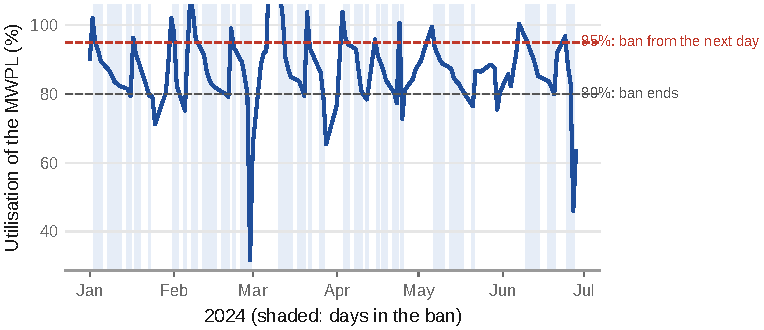
\includegraphics[width=\linewidth]{fig_util_example}
        \caption{Utilisation of the MWPL for SAIL, January to June 2024; shaded: ban days.}
      \end{figure}
    \end{column}
  \end{columns}
\end{frame}

\begin{frame}{Research question and objectives}
  \begin{block}{Research question}
    How strongly do limits to arbitrage bind in the Indian equity market, which of them matter, and how much mispricing
    do they explain?
  \end{block}
  \vspace{4pt}
  \begin{enumerate}
    \item Build one model in which every Indian limit is a parameter, and derive testable predictions with falsifiers.
    \item Freeze the tests before relating any outcome to any treatment.
    \item Measure mispricing (the futures-cash basis, earnings drift, price delay) from public exchange data.
    \item Test how bans, costs, capital, position limits and short-sale access shape mispricing.
    \item Draw out what the results imply for the regulation of position limits and short selling.
  \end{enumerate}
\end{frame}

\begin{frame}{Research gaps}
  \begin{table}
    \scriptsize
    \caption{Earlier Indian estimates of the futures-cash band}
    \begin{tabular}{@{}p{3.1cm}p{2.5cm}p{2.0cm}p{2.6cm}@{}}
      \toprule
      Study & Sample & Data & Band \\
      \midrule
      Aggarwal (2015) & 141 stocks, 2013 & One-second & $-15$ to $+3$\bp \\
      Shankar, Sankar and Kiran Kumar (2019) & 102 stocks, 2007 to 2009 & Five-minute & $-39$ to $-10$\bp \\
      Slivka, Shah and Wu (2011) & Cost calculation & Fee schedules & Twice mature markets \\
      \textbf{This study} & \textbf{360 stocks, 2015 to 2026} & \textbf{Daily} & $\mathbf{-34.5}$ to $\mathbf{+23.9}$\bp \\
      \bottomrule
    \end{tabular}
  \end{table}
  \begin{itemize}
    \small
    \item Earlier work measures intraday bands over short samples and never uses the ban.
    \item No study has estimated the effects of a reduce-only rule that binds every participant.
    \item Limits are usually studied one at a time, not side by side within one market.
  \end{itemize}
\end{frame}

\begin{frame}{Main contributions}
  \begin{enumerate}
    \item The first study of India's F\&O ban, modelled as a reduce-only rule for every participant.
    \item A model showing that the ban makes correction one-sided and its effect on the level of the basis ambiguous in
    sign; and that the position limit is not a valid instrument for ban status.
    \item Pre-registered tests with falsifiers, frozen with a time stamp; all results reported.
    \item Estimates of the no-arbitrage band over a long daily panel, related to dated changes in costs, capital and
    position limits.
    \item A constraint index for every listed Indian stock, released as a data set.
  \end{enumerate}
\end{frame}

%======================================================================================================================
\section{Background and Literature}

\begin{frame}{Why arbitrage is limited}
  \begin{itemize}
    \item \textbf{Capital:} arbitrageurs invest other people's money; losses bring withdrawals when gaps widen
    (Shleifer and Vishny, 1997).
    \item \textbf{Risk:} noise-trader risk deters short-horizon arbitrageurs (De Long et al., 1990); the result needs
    market-wide noise and is fragile (Loewenstein and Willard, 2006).
    \item \textbf{Costs and short sales:} a shorting cost makes the band one-sided (Gromb and Vayanos, 2010).
    \item \textbf{Short-sale constraints and prices:} overpricing (Miller, 1977); slower incorporation of bad news
    (Diamond and Verrecchia, 1987).
    \item \textbf{The band:} threshold and smooth-transition models of futures and cash (Dwyer, Locke and Yu, 1996;
    Tse, 2001; Ters and Urban, 2020).
  \end{itemize}
\end{frame}

%======================================================================================================================
\section{Institutional Setting}

\begin{frame}{Dated changes to the limits, 2015 to 2026}
  \begin{figure}
    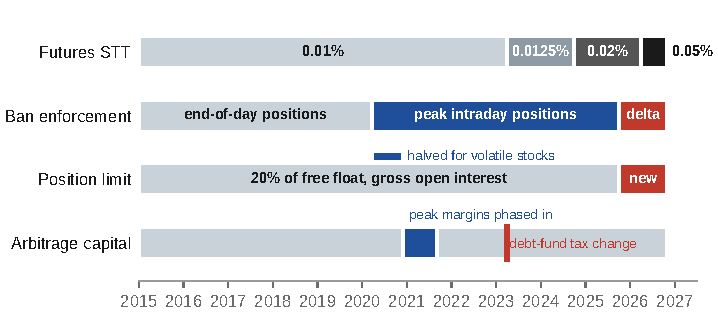
\includegraphics[width=\linewidth]{fig_timeline}
    \caption{Futures STT, enforcement of the ban, the position-limit rule and arbitrage capital.}
  \end{figure}
  \small
  \begin{itemize}
    \item To 22 March 2020 ban violations were judged on end-of-day positions; then on peak intraday positions; from
    October 2025 on end-of-day delta.
  \end{itemize}
\end{frame}

\begin{frame}{Position limits and short selling}
  \begin{table}
    \scriptsize
    \caption{The market-wide position limit over the sample}
    \begin{tabular}{@{}p{2.4cm}p{4.6cm}p{3.2cm}@{}}
      \toprule
      Period & MWPL & Open interest tested \\
      \midrule
      To 30 Sep 2025 & 20\% of free float & Gross, futures and options \\
      Mar to Nov 2020 & Halved for volatile or heavily used stocks & Gross \\
      From 1 Oct 2025 & Lower of 15\% of free float and 65 times average daily delivery; floor 10\% & Delta-adjusted \\
      \bottomrule
    \end{tabular}
  \end{table}
  \begin{itemize}
    \small
    \item Only F\&O stocks are eligible for short selling; naked shorting is barred; securities lending is thin.
    \item The practical overnight short is a single-stock future, so F\&O entry and exit change a stock's short-sale
    constraint at once.
  \end{itemize}
\end{frame}

%======================================================================================================================
\section{Theoretical Model}

\begin{frame}{Set-up}
  \begin{itemize}
    \item Basis $m=\ln F-\ln F^*$, with $F^*=(S-\mathrm{PV}(D))\,e^{r(T-t)}$.
    \item Outside traders create demand pressure $u$ toward futures; an arbitrage sector holds $a$ units of
    cash-and-carry. Market clearing:
    \[ m=\frac{u-a}{\Phi}. \]
    \item The sector maximises
    \[ \Pi(a)=a\,m-\tfrac{\gamma}{2}a^2-c_+a^+-c_-a^-,\qquad \gamma=\alpha\sigma^2, \]
    where $c_+$ is the cost of cash-and-carry and $c_-$ the cost of reverse arbitrage.
    \item Every Indian limit is a parameter: costs ($c_\pm$), short sales ($c_-$), capital and risk ($\gamma$),
    position limits (caps on $a$).
  \end{itemize}
\end{frame}

\begin{frame}{The no-arbitrage band}
  \begin{columns}[c]
    \begin{column}{0.5\textwidth}
      \begin{proposition}[Band]
        \small Arbitrage starts only when $m$ leaves $[-c_-,\,c_+]$. Inside, $\partial m/\partial u=1/\Phi$; outside,
        $\partial m/\partial u=\gamma/(\gamma\Phi+1)$.
      \end{proposition}
      \small
      \begin{itemize}
        \item Costs set the edges one for one
        \item Capital and risk set how far $m$ travels beyond them
        \item $c_->c_+$ in India: the band sits below zero
      \end{itemize}
    \end{column}
    \begin{column}{0.5\textwidth}
      \begin{figure}
        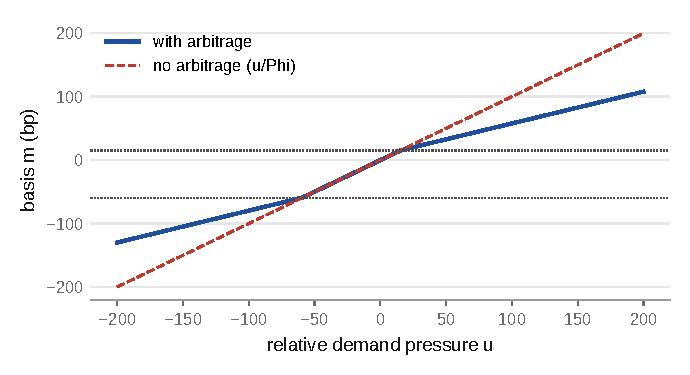
\includegraphics[width=\linewidth]{model_band}
        \caption{Equilibrium basis against demand pressure (illustrative costs).}
      \end{figure}
    \end{column}
  \end{columns}
\end{frame}

\begin{frame}{The F\&O ban as a reduce-only rule}
  \begin{assumption}[Ban]
    \small (B1) Arbitrageurs may only reduce: $0\le a_t\le a_{t-1}$. (B2) New futures demand is blocked; a share
    $\chi$ moves to the stock, the rest is withdrawn.
  \end{assumption}
  \begin{proposition}[One-sided correction]
    \small Rich futures are no longer corrected; cheap futures are, at a floor $\gamma a_t-c_u$ that wears out as
    positions are unwound.
  \end{proposition}
  \begin{proposition}[Level effect]
    \small The ban raises the basis when pressure comes from closing trades and lowers it when new demand keeps
    arriving: its sign is set by the composition of order flow.
  \end{proposition}
  {\scriptsize Further results: trading in a ban ($\Delta OI=-V$), anticipation below 95\%, the MWPL is not an
  instrument for bans, bad news is incorporated more slowly, Miller overpricing.}
\end{frame}

\begin{frame}{A simulated ban}
  \begin{figure}
    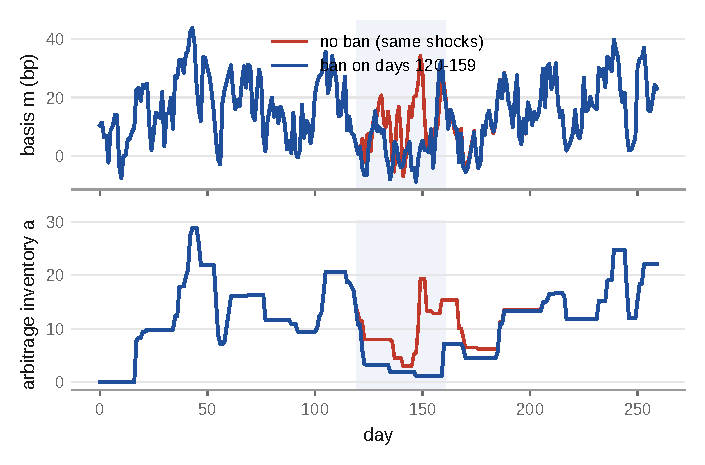
\includegraphics[width=0.82\linewidth]{model_path}
    \caption{Same shocks with and without a ban on days 120 to 159: basis (top) and arbitrage inventory (bottom).
    Illustrative parameters.}
  \end{figure}
\end{frame}

\begin{frame}{Hypotheses and falsifiers}
  \begin{table}
    \scriptsize
    \caption{Pre-specified hypotheses; the first four form the primary family (Holm correction)}
    \begin{tabular}{@{}p{0.9cm}p{6.0cm}p{3.4cm}@{}}
      \toprule
      & Prediction & Contradicted if \\
      \midrule
      \textbf{H8} & In a ban, futures volume falls and every trade closes positions & Futures activity unchanged \\
      \textbf{H7} & In a ban, rich futures revert more slowly & No asymmetry, or the opposite \\
      \textbf{H3} & Band edges move with the STT & Edges unrelated to costs \\
      \textbf{H6} & F\&O entry lowers price delay and bad-news drift & No change, or the opposite \\
      \midrule
      Level & The level effect follows the composition of open interest & Sign unrelated to composition \\
      H9 & The upper tail grows as utilisation nears 95\% & Jump only at 95\% \\
      H2, H1 & Bad news slower in bans; wider bands with frictions & Symmetric; no relation \\
      H4, H5 & Scarce capital widens the band; one-sided anomalies & No relation; symmetric \\
      \bottomrule
    \end{tabular}
  \end{table}
\end{frame}

%======================================================================================================================
\section{Data and Methodology}

\begin{frame}{Data}
  \begin{table}
    \scriptsize
    \caption{Public data sources}
    \begin{tabular}{@{}p{3.6cm}p{4.6cm}p{2.0cm}@{}}
      \toprule
      Source & Content & Coverage \\
      \midrule
      NSE open interest, ban lists & MWPL, open interest, ban status & 2010 to 2026 \\
      NSE bhavcopies, delivery files & Futures and cash prices, volumes, delivery & 2015 to 2026 \\
      NSE corporate events & Dividends, splits, results dates & 2014 to 2026 \\
      NSE securities lending & Daily lending trades and fees & 2015 to 2026 \\
      AMFI & Market capitalisation; arbitrage-fund flows & 2017 to 2026 \\
      \bottomrule
    \end{tabular}
  \end{table}
  \begin{exampleblock}{Checks}
    \small Next-day flags match the official ban list for 99.9\% of flags; results are dated from the exchange's first
    dissemination time; a full rerun reproduces every number.
  \end{exampleblock}
\end{frame}

\begin{frame}{The futures-cash basis}
  \[ m_{it}=\ln\bar F_{it}-\ln\big(\bar S_{it}-\mathrm{PV}_{it}(D)\big)-r_t\tau_{it} \]
  \vspace{-6pt}
  \begin{columns}[c]
    \begin{column}{0.4\textwidth}
      \scriptsize
      \begin{itemize}
        \item Volume-weighted prices, not settlement prices (set at cost of carry on thin days)
        \item Near-month contract, at least 5 contracts traded, no dividend in its life
        \item 486,040 stock-days, 371 stocks
      \end{itemize}
    \end{column}
    \begin{column}{0.6\textwidth}
      \begin{figure}
        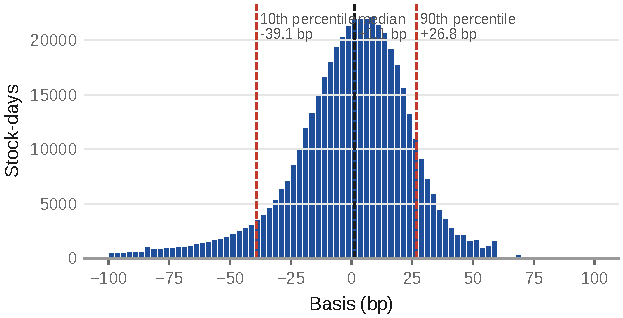
\includegraphics[width=\linewidth]{fig_basis_dist}
        \caption{Distribution of the basis (bp).}
      \end{figure}
    \end{column}
  \end{columns}
\end{frame}

\begin{frame}{Research design}
  \centering
  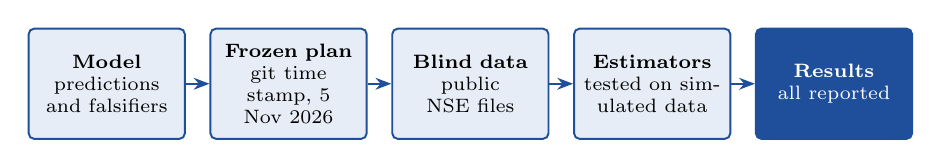
\begin{tikzpicture}[node distance=3mm,
    box/.style={draw=iitbblue,line width=0.7pt,rounded corners=2pt,fill=iitblight,text width=1.75cm,minimum height=1.4cm,align=center,font=\scriptsize},
    arr/.style={-{Stealth[length=2mm]},line width=0.8pt,color=iitbblue}]
    \node[box] (a) {\textbf{Model}\\ predictions and falsifiers};
    \node[box,right=of a] (b) {\textbf{Frozen plan}\\ git time stamp, 5 Nov 2026};
    \node[box,right=of b] (c) {\textbf{Blind data}\\ public NSE files};
    \node[box,right=of c] (d) {\textbf{Estimators}\\ tested on simulated data};
    \node[box,right=of d,fill=iitbblue,text=white] (e) {\textbf{Results}\\ all reported};
    \foreach \x/\y in {a/b,b/c,c/d,d/e} \draw[arr] (\x) -- (\y);
  \end{tikzpicture}
  \vspace{8pt}
  \begin{itemize}
    \small
    \item \textbf{Estimators:} two-way fixed effects with clustered errors; threshold and smooth-transition models;
    matched event studies; density test and regression discontinuity; Callaway and Sant'Anna difference-in-differences.
    \item \textbf{Inference:} primary family Holm-corrected at 5\%; secondary tests unadjusted and read as a pattern.
  \end{itemize}
\end{frame}

%======================================================================================================================
\section{Results I: The F\&O Ban}

\begin{frame}{Trading in a ban (H8)}
  \begin{table}
    \scriptsize
    \caption{Ban days against the same stock's non-ban days at 80 to 95\% utilisation}
    \begin{tabular}{lcc}
      \toprule
      Outcome & Effect (s.e.) & Non-ban mean \\
      \midrule
      log(1 + futures contracts) & $-2.00$ (0.11) & \\
      log(1 + cash shares) & $+0.073$ (0.027) & \\
      Delivery share & $+0.041$ (0.005) & 0.26 \\
      \bottomrule
    \end{tabular}
  \end{table}
  \vspace{-4pt}
  \begin{figure}
    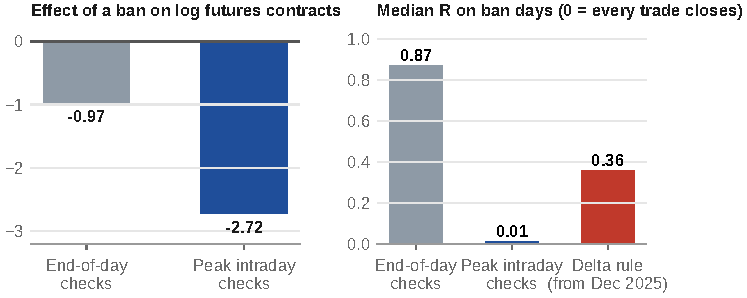
\includegraphics[width=0.82\linewidth]{fig_h8_era}
    \caption{By enforcement regime: futures effect (left) and median $R=(\Delta OI+V)/V$ on ban days (right).}
  \end{figure}
\end{frame}

\begin{frame}{Enforcement decides whether the rule binds}
  \begin{figure}
    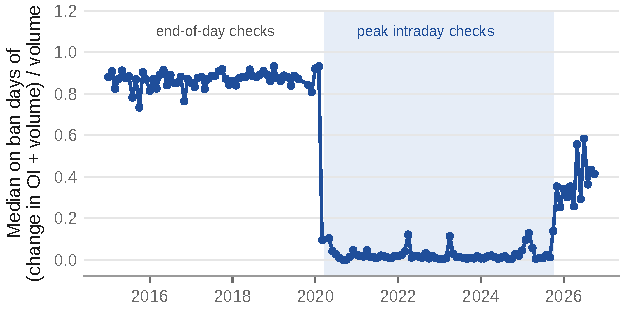
\includegraphics[width=0.88\linewidth]{fig_ban_R}
    \caption{Monthly median of $R$ on ban days; $R=0$ when every trade closes a long and a short.}
  \end{figure}
  \keybox{Under intraday checks (March 2020 to September 2025) the median $R$ is 0.011: every trade in a ban closed
  positions.}
\end{frame}

\begin{frame}{Does correction become one-sided? (H7)}
  \begin{columns}[c]
    \begin{column}{0.42\textwidth}
      \begin{table}
        \scriptsize
        \caption{Reversion slopes}
        \begin{tabular}{lcc}
          \toprule
          & Normal & Change in ban \\
          \midrule
          Upper & $-0.712$ & $\mathbf{-0.089}$ \\
          Middle & $-0.393$ & $+0.099$ \\
          Lower & $-0.204$ & $\mathbf{+0.081}$ \\
          \bottomrule
        \end{tabular}
      \end{table}
      \begin{alertblock}{Prediction rejected}
        \scriptsize Rich futures revert \emph{faster} in a ban, mostly in the first five days of a spell.
      \end{alertblock}
    \end{column}
    \begin{column}{0.58\textwidth}
      \begin{figure}
        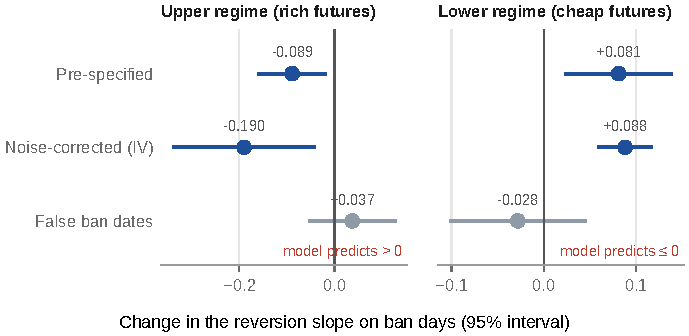
\includegraphics[width=\linewidth]{fig_h7_dots}
        \caption{Change in slope: pre-specified, noise-corrected, false ban dates.}
      \end{figure}
    \end{column}
  \end{columns}
\end{frame}

\begin{frame}{The level of the basis when a ban starts}
  \begin{columns}[c]
    \begin{column}{0.6\textwidth}
      \begin{figure}
        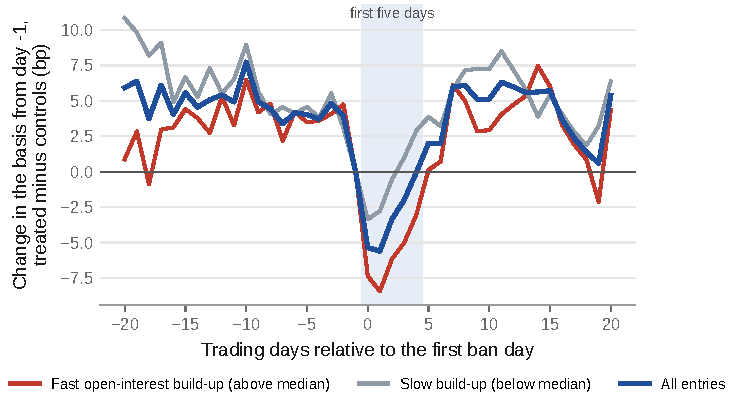
\includegraphics[width=\linewidth]{fig_level_profile}
        \caption{Treated minus matched controls, by event day (889 entries).}
      \end{figure}
    \end{column}
    \begin{column}{0.4\textwidth}
      \scriptsize
      \begin{itemize}
        \item Basis falls by 6.3\bp\ in the first days; returns after about a week
        \item Rising open interest before entry: $-6.8$\bp; falling: $+8.4$\bp\ (30 events)
        \item Difference $-15.2$\bp\ ($p=0.083$); median split $p=0.025$
        \item Same for long and short build-ups; nothing at false entries
      \end{itemize}
    \end{column}
  \end{columns}
  \keybox{Consistent with blocked new futures demand (a reading formed after the results).}
\end{frame}

\begin{frame}{The 95\% trigger: no bunching}
  \begin{figure}
    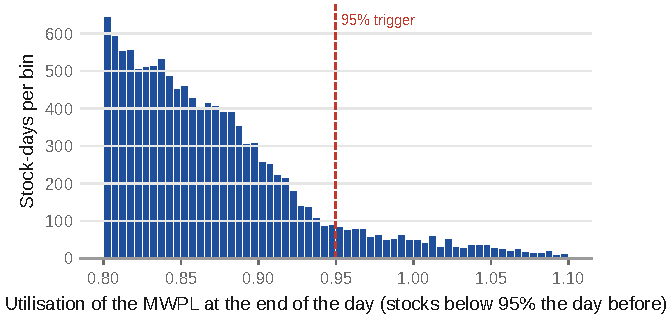
\includegraphics[width=0.78\linewidth]{fig_density}
    \caption{End-of-day utilisation of stocks that were below 95\% the day before, 2015 to September 2025.}
  \end{figure}
  \footnotesize
  \begin{itemize}
    \item Cattaneo, Jansson and Ma test: $T=-0.18$, $p=0.86$; robust to bandwidth, order and enforcement period.
    \item Utilisation accelerates rather than stalls near the trigger: traders do not hold back.
  \end{itemize}
\end{frame}

\begin{frame}{The 95\% trigger: regression discontinuity}
  \begin{figure}
    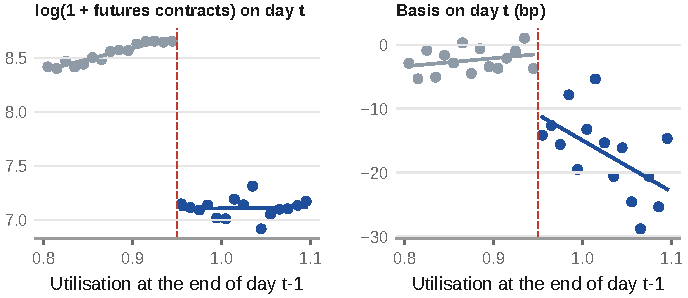
\includegraphics[width=0.84\linewidth]{fig_rd}
    \caption{Binned means by utilisation at the end of the previous day, stocks not in a ban the day before.}
  \end{figure}
  \footnotesize
  \begin{itemize}
    \item Futures trading drops by 1.53 log points at 95\%; $R$ falls by 0.66; delivery share rises.
    \item The basis is 12.9\bp\ lower above the cutoff, but already 11.3\bp\ lower on the crossing day.
    \item Hysteresis (80 to 95\%): being in a ban adds $+0.4$\bp\ ($p=0.64$).
  \end{itemize}
\end{frame}

%======================================================================================================================
\section{Results II: Costs, Capital and Position Limits}

\begin{frame}{The no-arbitrage band}
  \begin{columns}[c]
    \begin{column}{0.5\textwidth}
      \begin{figure}
        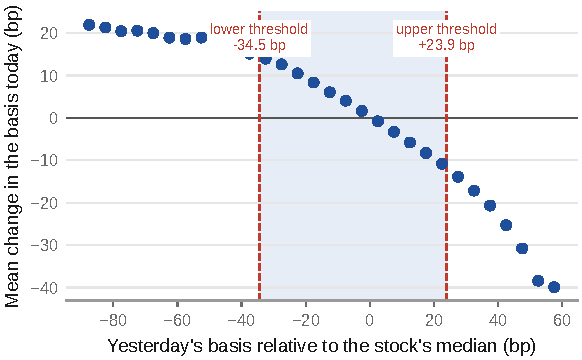
\includegraphics[width=\linewidth]{fig_band_scatter}
        \caption{Mean daily change by yesterday's deviation.}
      \end{figure}
    \end{column}
    \begin{column}{0.5\textwidth}
      \begin{table}
        \scriptsize
        \caption{Pooled threshold model}
        \begin{tabular}{lccc}
          \toprule
          & Lower & Middle & Upper \\
          \midrule
          Threshold & $-34.5$ & & $+23.9$ \\
          Slope & $-0.084$ & $-0.468$ & $-0.809$ \\
          IV slope & $-0.121$ & $-0.192$ & $-0.141$ \\
          \bottomrule
        \end{tabular}
      \end{table}
      \scriptsize Linearity rejected (sup-$F$ 7,471). Instrumenting shows most daily reversion is price noise.
    \end{column}
  \end{columns}
\end{frame}

\begin{frame}{Costs and the band (H3)}
  \begin{figure}
    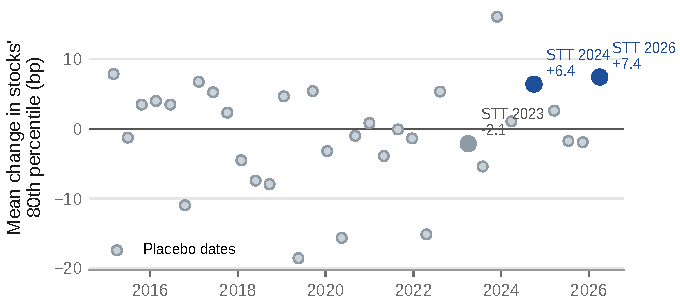
\includegraphics[width=0.8\linewidth]{fig_h3_placebo}
    \caption{Mean change in stocks' 80th percentile of the basis at the STT dates and at 30 placebo dates (bp).}
  \end{figure}
  \footnotesize
  \begin{itemize}
    \item Pre-specified: $+6.96$\bp\ (s.e.\ 0.61) pooling 2024 and 2026; ordering 2026 $>$ 2024 $>$ 2023 holds.
    \item But the placebo s.d.\ is 7.4\bp: the rise is mostly a common shift, larger than the cost changes.
  \end{itemize}
\end{frame}

\begin{frame}{The cost of a new cash-and-carry position}
  \begin{figure}
    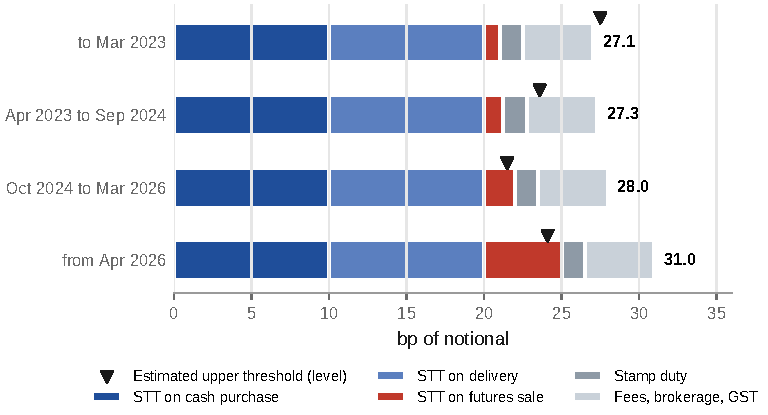
\includegraphics[width=0.8\linewidth]{fig_cost_band}
    \caption{Round trip of an overnight position held to delivery, by STT period (bp of notional).}
  \end{figure}
  \footnotesize
  \begin{itemize}
    \item A new round trip costs 27 to 31\bp, above the estimated upper edge; rolling costs only 4 to 8\bp.
    \item New capital enters only at large gaps; funds that roll lean against small ones.
  \end{itemize}
\end{frame}

\begin{frame}{Arbitrage capital (H4)}
  \begin{figure}
    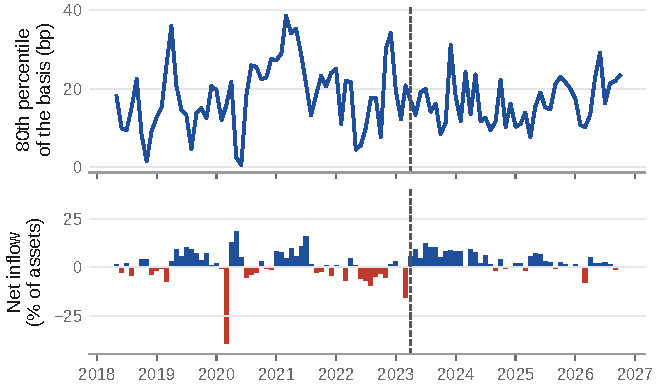
\includegraphics[width=0.62\linewidth]{fig_h4_flows}
    \caption{Monthly 80th percentile of the basis (top) and net inflow into arbitrage funds (bottom).}
  \end{figure}
  \footnotesize
  \begin{itemize}
    \item $-17.5$\bp\ per unit of lagged flow ($p=0.11$); clearer in first differences ($-20.6$, s.e.\ 6.8).
    \item Visible before April 2023, not after, when assets grew fastest.
  \end{itemize}
\end{frame}

\begin{frame}{Anticipation below the trigger (H9)}
  \begin{figure}
    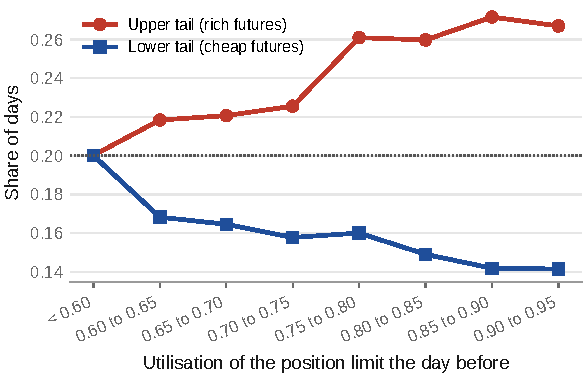
\includegraphics[width=0.72\linewidth]{fig_h9_tails}
    \caption{Share of non-ban days in the stock's upper and lower tail, by utilisation the day before.}
  \end{figure}
  \footnotesize
  \begin{itemize}
    \item Upper-tail share rises from 0.20 to 0.27 toward 95\% ($p=0.019$); the lower tail is flat with date effects.
    \item October 2025 reform: right direction, not significant ($p=0.11$).
  \end{itemize}
\end{frame}

\begin{frame}{Restoring the position limit in 2020}
  \begin{figure}
    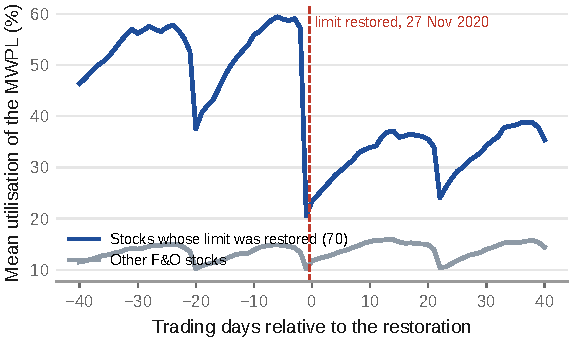
\includegraphics[width=0.72\linewidth]{fig_covid}
    \caption{Mean utilisation of the 70 stocks whose halved limit was restored on 27 November 2020, and of others.}
  \end{figure}
  \footnotesize
  \begin{itemize}
    \item Utilisation $-0.21$, ban days $-4.6$ points, upper tail $-6.8$ points; level unchanged.
    \item A looser limit made rich futures less common, as the anticipation result predicts.
  \end{itemize}
\end{frame}

\begin{frame}{The 2025 rules and ``spurious'' bans}
  \begin{figure}
    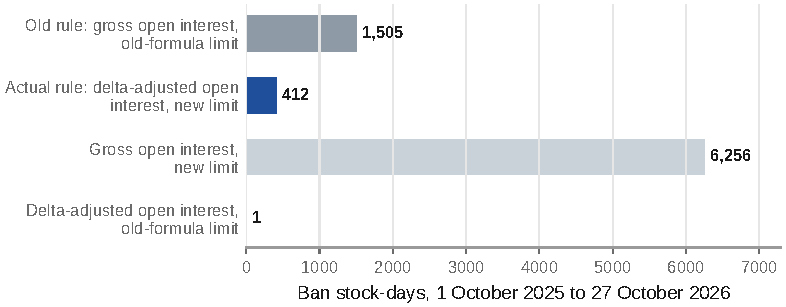
\includegraphics[width=0.72\linewidth]{fig_spurious}
    \caption{Ban stock-days, 1 October 2025 to 27 October 2026, under the actual and three counterfactual rules.}
  \end{figure}
  \footnotesize
  \begin{itemize}
    \item Before 2025 bans came from rising open interest; only 0.4\% from a falling limit.
    \item Delta-adjusted open interest removes almost all bans; the lower limit alone would have quadrupled them.
  \end{itemize}
  \keybox{412 ban days against 1,505 under the old rule: about three quarters fewer.}
\end{frame}

%======================================================================================================================
\section{Results III: Short-Sale Constraints}

\begin{frame}{Entry into and exit from the F\&O segment (H6)}
  \begin{columns}[c]
    \begin{column}{0.56\textwidth}
      \begin{figure}
        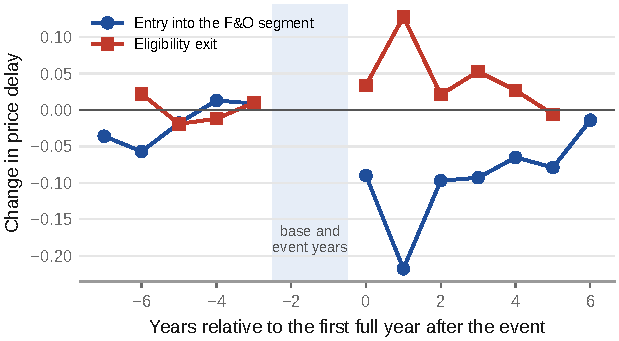
\includegraphics[width=\linewidth]{fig_h6_es}
        \caption{Change in price delay by year relative to the event.}
      \end{figure}
    \end{column}
    \begin{column}{0.44\textwidth}
      \begin{table}
        \scriptsize
        \caption{Pre-specified components}
        \begin{tabular}{lcc}
          \toprule
          & Estimate & $p$ \\
          \midrule
          Entry: delay & $\mathbf{-0.109}$ & $10^{-6}$ \\
          Entry: drift & $-0.040$ & 0.99 \\
          Exit: delay & $+0.053$ & 0.09 \\
          Exit: drift & $+0.014$ & 0.77 \\
          \bottomrule
        \end{tabular}
      \end{table}
      \scriptsize Sun and Abraham: $-0.063$ (s.e.\ 0.019). Selection on growth cannot be ruled out.
    \end{column}
  \end{columns}
\end{frame}

\begin{frame}{A constraint index for every listed stock}
  \begin{figure}
    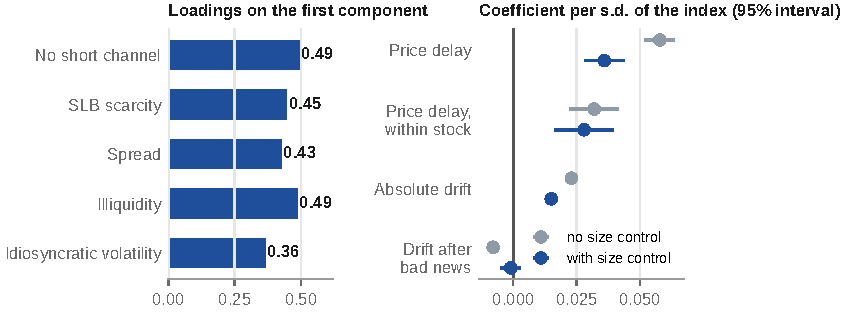
\includegraphics[width=\linewidth]{fig_index}
    \caption{Loadings of five frictions on the first component (left); validation with and without a size control
    (right). 80,042 stock-quarters, 3,310 stocks.}
  \end{figure}
  \small
  \begin{itemize}
    \item More constrained stocks adjust more slowly, also within stocks and after a size control.
    \item The index's link with drift after bad news disappears once size is controlled for.
  \end{itemize}
\end{frame}

\begin{frame}{Anomalies and short-sale constraints (H5)}
  \begin{figure}
    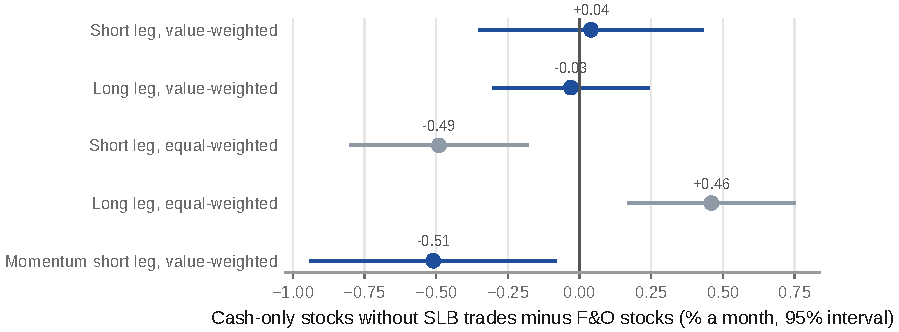
\includegraphics[width=0.9\linewidth]{fig_h5_legs}
    \caption{Cash-only stocks without lending minus F\&O stocks, legs of a composite mispricing sort.}
  \end{figure}
  \small
  \begin{itemize}
    \item Value-weighted, the overpriced side does no worse where shorting is hardest ($p=0.57$).
    \item Equal-weighted, anomalies are stronger among small cash-only stocks, on both sides; momentum alone fits.
  \end{itemize}
\end{frame}

%======================================================================================================================
\section{Conclusions and Future Scope}

\begin{frame}{Summary of the pre-specified tests}
  \begin{table}
    \scriptsize
    \begin{tabular}{@{}p{3.6cm}p{3.0cm}p{3.6cm}@{}}
      \toprule
      Hypothesis & Result & Comment \\
      \midrule
      H8 trading & \textcolor{okgreen}{Supported} & Identity holds under intraday checks \\
      H3 costs & \textcolor{okgreen}{Supported} & Weak against placebos \\
      H6 short-sale access & \textcolor{okgreen}{Supported} & Through price delay only \\
      H7 one-sided correction & \textcolor{alertred}{Rejected, opposite sign} & Survives a noise correction \\
      \midrule
      Level effect & $p=0.083$ & Signs as predicted \\
      Density, RD at 95\% & $p=0.86$; $-12.9$\bp & Gap before the ban \\
      Hysteresis & $p=0.64$ & No extra level shift \\
      H9 anticipation, reform & $p=0.019$; $p=0.11$ & Right direction \\
      H2, H1, H4, H5 & $p=0.59$, 0.002, 0.11, 0.57 & Mixed \\
      \bottomrule
    \end{tabular}
  \end{table}
\end{frame}

\begin{frame}{Conclusions}
  \begin{itemize}
    \item \textbf{Position limits} bind hard on trading; their price effect is real but not the predicted one-sided
    correction, and it fades within a week.
    \item \textbf{Enforcement} matters: the rule binds trade by trade only under intraday checks.
    \item \textbf{Short-sale access} speeds price adjustment, but evidence on overpricing and bad-news drift is mixed.
    \item \textbf{Trading costs} shape a wide, asymmetric band; its edges do not move one for one with the tax.
    \item \textbf{Arbitrage capital} leaves weak traces in the predicted direction.
  \end{itemize}
\end{frame}

\begin{frame}{Policy implications}
  \begin{columns}[T]
    \begin{column}{0.5\textwidth}
      \begin{block}{What the evidence shows}
        \scriptsize
        \begin{itemize}
          \item A ban cuts futures volume by almost 90\%
          \item Its price effect appears at ban start and fades
          \item The 2025 rules cut ban days by three quarters
        \end{itemize}
      \end{block}
    \end{column}
    \begin{column}{0.5\textwidth}
      \begin{block}{What it implies}
        \scriptsize
        \begin{itemize}
          \item Bans restrain speculative demand at the cost of arbitrage
          \item Enforcement matters as much as the threshold
          \item Delta-based open interest removes avoidable bans
        \end{itemize}
      \end{block}
    \end{column}
  \end{columns}
  \vspace{6pt}
  \small SEBI's study: 93\% of more than one crore individual F\&O traders lost money over FY22 to FY24 (SEBI, 2024a).
  The demand that position limits restrain is large.
\end{frame}

\begin{frame}{Limitations and future scope}
  \begin{columns}[T]
    \begin{column}{0.5\textwidth}
      \begin{alertblock}{Limitations}
        \scriptsize
        \begin{itemize}
          \item Daily data: noise inflates measured reversion
          \item Arbitrage inventory is not observed
          \item Only 44 ban spells since October 2025
          \item Size confounds cross-sectional comparisons
        \end{itemize}
      \end{alertblock}
    \end{column}
    \begin{column}{0.5\textwidth}
      \begin{exampleblock}{Future scope}
        \scriptsize
        \begin{itemize}
          \item Intraday data for sharper tests of correction in bans
          \item A longer post-reform sample for the 2025 formula
          \item Extend the model for blocked new demand
          \item Observed-state smooth-transition models of the band
        \end{itemize}
      \end{exampleblock}
    \end{column}
  \end{columns}
\end{frame}

\begin{frame}[allowframebreaks]{Important references}
  \tiny
  \begin{thebibliography}{99}
    \bibitem{agg} Aggarwal, N. (2015). Limits to arbitrage: The case of single stock futures and spot prices. IGIDR WP-2015-010.
    \bibitem{cs} Callaway, B. and P. Sant'Anna (2021). Difference-in-differences with multiple time periods. \emph{J. Econometrics} 225(2).
    \bibitem{dssw} De Long, J. B., A. Shleifer, L. Summers and R. Waldmann (1990). Noise trader risk in financial markets. \emph{J. Political Economy} 98(4).
    \bibitem{dv} Diamond, D. and R. Verrecchia (1987). Constraints on short-selling and asset price adjustment to private information. \emph{J. Financial Economics} 18(2).
    \bibitem{dly} Dwyer, G., P. Locke and W. Yu (1996). Index arbitrage and nonlinear dynamics between the S\&P 500 futures and cash. \emph{Rev. Financial Studies} 9(1).
    \bibitem{gv} Gromb, D. and D. Vayanos (2010). Limits of arbitrage. \emph{Annual Rev. Financial Economics} 2.
    \bibitem{hm} Hou, K. and T. Moskowitz (2005). Market frictions, price delay, and the cross-section of expected returns. \emph{Rev. Financial Studies} 18(3).
    \bibitem{lw} Loewenstein, M. and G. Willard (2006). The limits of investor behavior. \emph{J. Finance} 61(1).
    \bibitem{mil} Miller, E. (1977). Risk, uncertainty, and divergence of opinion. \emph{J. Finance} 32(4).
    \bibitem{ssa} Saurav, S., P. Srivastava and S. K. Agarwalla (2026). Decoupled: Disagreement, short-sale constraints, and law-of-one-price violations around earnings announcements. SSRN.
    \bibitem{sebi} SEBI (2024a). Press release 22/2024 on profits and losses of individual F\&O traders; SEBI (2025). Circular SEBI/HO/MRD/TPD-1/P/CIR/2025/79.
    \bibitem{ssk} Shankar, R. L., G. Sankar and K. Kiran Kumar (2019). Mispricing in single stock futures: Empirical examination of Indian markets. \emph{Emerging Markets Finance and Trade} 55(7).
    \bibitem{sv} Shleifer, A. and R. Vishny (1997). The limits of arbitrage. \emph{J. Finance} 52(1).
    \bibitem{syy} Stambaugh, R., J. Yu and Y. Yuan (2015). Arbitrage asymmetry and the idiosyncratic volatility puzzle. \emph{J. Finance} 70(5).
    \bibitem{tu} Ters, K. and J. Urban (2020). Estimating unknown arbitrage costs: Evidence from a 3-regime threshold vector error correction model. \emph{J. Financial Markets} 47.
    \bibitem{tse} Tse, Y. (2001). Index arbitrage with heterogeneous investors: A smooth transition error-correction analysis. \emph{J. Banking and Finance} 25(10).
  \end{thebibliography}
\end{frame}

\begin{frame}{Acknowledgement}
  I thank my supervisor, Prof.\ Aditi Chaubal, for her guidance throughout this project, and in particular for the
  advice to build a formal model of what the project would test before looking at any data.
\end{frame}

\begin{frame}
  \centering
  {\Huge\color{iitbblue} Thank You}\\[12pt]
  {\small Questions and comments are welcome}
\end{frame}

%======================================================================================================================
\appendix
\section*{Backup Slides}

\begin{frame}{Backup: the model's results and the tests}
  \begin{table}
    \scriptsize
    \begin{tabular}{@{}p{2.6cm}p{5.6cm}p{2.0cm}@{}}
      \toprule
      Result & Statement & Tested by \\
      \midrule
      Band, comparative statics & Arbitrage only outside $[-c_-,c_+]$; costs set the edges & H3, H4 \\
      Inventory & The no-trade region moves with the existing book & Estimator tests \\
      One-sided correction & In a ban, rich futures are not corrected & H7 \\
      Demand reversal, level & Blocked demand moves to cash; level sign not fixed & Level effect \\
      Trading & Contract-level enforcement: $\Delta OI=-V$ & H8 \\
      Anticipation, identification & Upper edge rises toward 95\%; MWPL not an instrument & H9, density, RD \\
      Short sales & Bad news slower without a short channel; Miller & H2, H5, H6 \\
      \bottomrule
    \end{tabular}
  \end{table}
\end{frame}

\begin{frame}{Backup: bans over time}
  \begin{figure}
    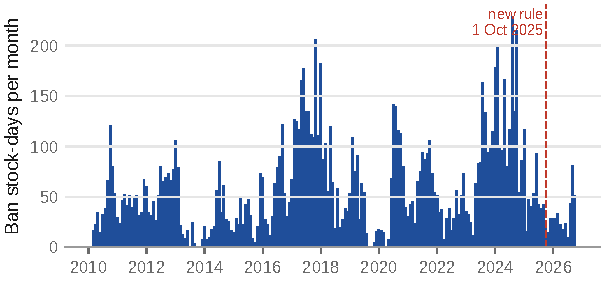
\includegraphics[width=\linewidth]{fig_ban_month}
    \caption{Stock-days in the ban per month, 2010 to 2026.}
  \end{figure}
\end{frame}

\begin{frame}{Backup: the October 2025 cut in the position limit}
  \begin{figure}
    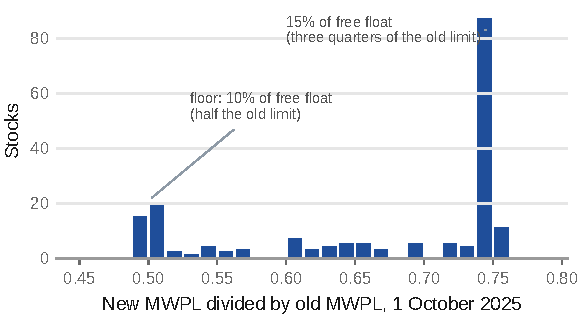
\includegraphics[width=0.9\linewidth]{fig_mwpl_ratio}
    \caption{New MWPL divided by old MWPL, 1 October 2025 (208 stocks).}
  \end{figure}
\end{frame}

\begin{frame}{Backup: level effect by group}
  \begin{figure}
    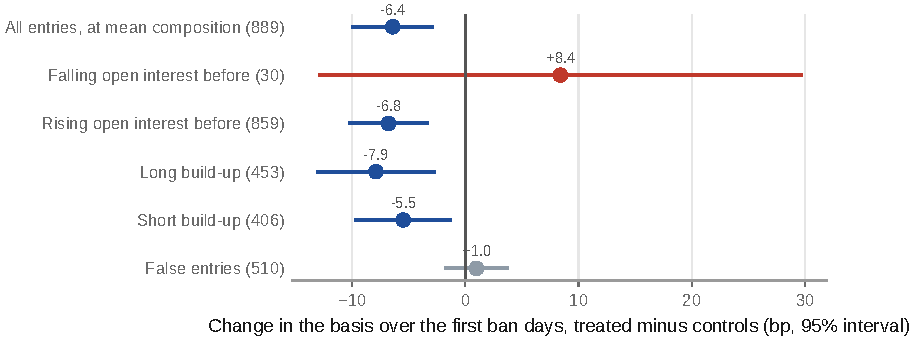
\includegraphics[width=0.95\linewidth]{fig_level_groups}
    \caption{Change in the basis over the first ban days, treated minus controls, by composition and build-up type,
    with false entries.}
  \end{figure}
\end{frame}

\begin{frame}{Backup: the pre-analysis plan and its log}
  \small
  \begin{itemize}
    \item Frozen with a git tag on 5 November 2026, after the supervisor's go-ahead and a full data audit; until then
    no outcome was related to any treatment.
    \item Every detail the plan left open (sample filters, composition splits, density population, outcome windows)
    was fixed in a dated log before the test that needed it.
    \item Analyses added after seeing a result are labelled exploratory; the pre-specified result is always reported
    first.
    \item Each estimator first recovered known effects on simulated data: the threshold model, the Callaway and
    Sant'Anna estimator and the matched level-effect design.
  \end{itemize}
\end{frame}

\end{document}
